\documentclass[12pt,a4paper]{article}
\usepackage[utf8]{inputenc}
\usepackage[T1]{fontenc}
\usepackage[french]{babel}
\usepackage{geometry}
\usepackage{graphicx}
\usepackage{xcolor}
\usepackage{titlesec}
\usepackage{fancyhdr}
\usepackage{hyperref}
\usepackage{float}
\geometry{margin=2.5cm}

\definecolor{bleu}{HTML}{2B6CB0}

\titleformat{\section}
  {\Large\bfseries\color{bleu}}{\thesection.}{0.4em}{}

\titleformat{\subsection}
  {\large\bfseries\color{bleu}}{\thesubsection}{0.4em}{}

\pagestyle{fancy}
\fancyhf{}
\fancyhead[L]{\small Maquettes — Nexora}
\fancyhead[R]{\small EMSI 2025-2026}
\fancyfoot[C]{\thepage}

\hypersetup{colorlinks=true, linkcolor=bleu, urlcolor=bleu}

\begin{document}

% ══════════════════════════════════════════════════════════════
\begin{titlepage}
\centering
\vspace*{1cm}

\includegraphics[width=0.5\textwidth]{emsilogo.png}\\[2cm]

\rule{\linewidth}{0.4pt}\\[0.4cm]
{\Large\textbf{Maquettes de l'Application}}\\[0.3cm]
{\Huge\bfseries\color{bleu} NEXORA}\\[0.3cm]
{\large\textit{Plateforme d'Intelligence Organisationnelle}}\\[0.3cm]
\rule{\linewidth}{0.4pt}

\vspace{2cm}

\begin{tabular}{cc}
    \multicolumn{2}{c}{\large\textbf{Réalisé par :}} \\[0.3cm]
    Soubaibi Omar & Yassine Baizi \\[1cm]
    \multicolumn{2}{c}{\large\textbf{Encadré par :}} \\[0.3cm]
    \multicolumn{2}{c}{Mme. OUNACER SOUMAYA} \\
\end{tabular}

\vfill
\textbf{Filière :} 4IADM G5-A \\[0.2cm]
\textbf{Année Universitaire :} 2025--2026
\end{titlepage}

\tableofcontents
\newpage

% ══════════════════════════════════════════════════════════════
\section{Introduction}
% ══════════════════════════════════════════════════════════════

Ce document présente les maquettes de toutes les interfaces de la plateforme Nexora. Chaque écran est accompagné d'un wireframe, d'une description, de ses composants et de ses interactions.

\textbf{Charte graphique :}
\begin{itemize}
    \item Fond principal : bleu sombre (\texttt{\#0F172A})
    \item Couleur d'accent : orange (\texttt{\#F97316})
    \item Composants UI : Material UI (MUI)
    \item Police : Roboto / Inter
\end{itemize}

% ══════════════════════════════════════════════════════════════
\section{Page de Connexion (Login)}
% ══════════════════════════════════════════════════════════════

\begin{figure}[H]
    \centering
    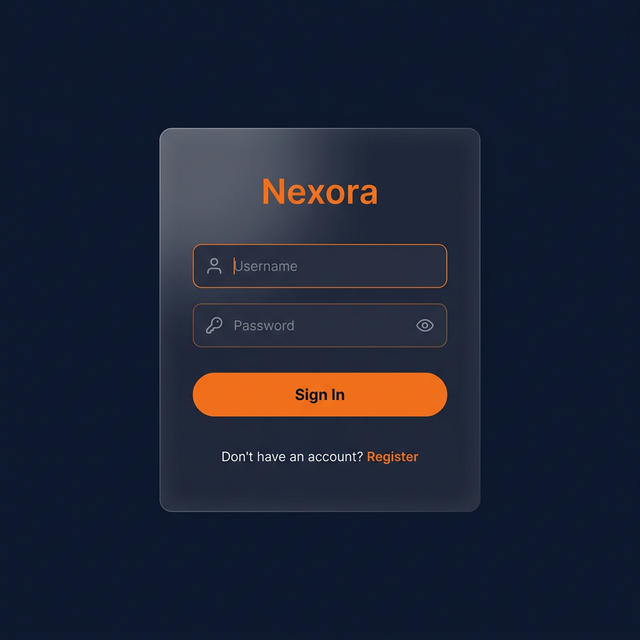
\includegraphics[width=0.85\textwidth]{maquettes/maquette_login.png}
    \caption{Page de connexion Nexora}
\end{figure}

\textbf{Description :} Première page visible. Toutes les autres pages redirigent ici si l'utilisateur n'est pas authentifié.

\textbf{Composants :}
\begin{itemize}
    \item Logo Nexora centré en haut de la carte.
    \item Champ \textit{Username} — identifiant de l'utilisateur.
    \item Champ \textit{Password} — mot de passe (masqué).
    \item Bouton \textbf{Sign In} en orange — déclenche l'authentification JWT.
    \item Lien \textit{Don't have an account? Register} — redirige vers l'inscription.
\end{itemize}

\textbf{Interactions :}
\begin{itemize}
    \item Appel POST \texttt{/api/auth/login}.
    \item Succès : stockage du token JWT, redirection vers le Feed.
    \item Erreur : message d'erreur (identifiants invalides, rate limit 5 tentatives/5 min).
\end{itemize}

% ══════════════════════════════════════════════════════════════
\section{Page d'Inscription (Register)}
% ══════════════════════════════════════════════════════════════

\begin{verbatim}
  ┌──────────────────────────────────────────────┐
  │                  NEXORA                      │
  │            Create your account               │
  │                                              │
  │  ┌────────────────────────────────────────┐  │
  │  │  Username                              │  │
  │  └────────────────────────────────────────┘  │
  │  ┌────────────────────────────────────────┐  │
  │  │  Email                                 │  │
  │  └────────────────────────────────────────┘  │
  │  ┌────────────────────────────────────────┐  │
  │  │  Password                              │  │
  │  └────────────────────────────────────────┘  │
  │  ┌────────────────────────────────────────┐  │
  │  │  Confirm Password                      │  │
  │  └────────────────────────────────────────┘  │
  │                                              │
  │  ┌────────────────────────────────────────┐  │
  │  │          REGISTER (orange)             │  │
  │  └────────────────────────────────────────┘  │
  │      Already have an account? Sign In        │
  └──────────────────────────────────────────────┘
\end{verbatim}

\textbf{Description :} Page d'inscription avec le même style que le login (carte centrée, glassmorphism).

\textbf{Composants :}
\begin{itemize}
    \item Champ \textit{Username} — vérifié pour unicité.
    \item Champ \textit{Email} — format validé.
    \item Champ \textit{Password} — minimum 4 caractères.
    \item Champ \textit{Confirm Password} — doit correspondre.
    \item Bouton \textbf{Register} en orange.
\end{itemize}

\textbf{Interactions :} POST \texttt{/api/auth/register}. Succès : redirection vers Login. Erreur : username/email déjà pris.

% ══════════════════════════════════════════════════════════════
\section{Feed (Fil d'Actualités)}
% ══════════════════════════════════════════════════════════════

\begin{verbatim}
  ┌──────────┬───────────────────────────────────┐
  │ SIDEBAR  │                                   │
  │          │ ┌─────────────────────────────┐   │
  │ Feed  *  │ │ Quoi de neuf ?     [Publier]│   │
  │ Network  │ └─────────────────────────────┘   │
  │ Jobs     │                                   │
  │ Messages │ ┌─────────────────────────────┐   │
  │ SkillMap │ │ [Av] Sarah Chen     2h ago  │   │
  │ Graph    │ │ Just completed the ML       │   │
  │ AI       │ │ pipeline for Project Nexus! │   │
  │ SkillEvo │ │ [Image]                     │   │
  │ Workspace│ │ ♥ 12   💬 3   Share         │   │
  │ Dashboard│ └─────────────────────────────┘   │
  │          │                                   │
  │          │ ┌─────────────────────────────┐   │
  │          │ │ [Av] Omar S.        5h ago  │   │
  │          │ │ New article on Graph DBs    │   │
  │          │ │ ♥ 8    💬 1   Share          │   │
  │          │ └─────────────────────────────┘   │
  └──────────┴───────────────────────────────────┘
\end{verbatim}

\textbf{Description :} Page principale après connexion, inspirée de LinkedIn. Publications multimédia avec interactions sociales.

\textbf{Composants :}
\begin{itemize}
    \item \textbf{Zone de publication} — champ texte + bouton photo + publier.
    \item \textbf{Carte de publication} — avatar, nom, date, contenu, image, actions (Like, Comment, Share).
    \item \textbf{Sidebar} — navigation globale, présente sur toutes les pages.
\end{itemize}

% ══════════════════════════════════════════════════════════════
\section{My Network (Réseau)}
% ══════════════════════════════════════════════════════════════

\begin{verbatim}
  ┌──────────┬───────────────────────────────────┐
  │ SIDEBAR  │ My Network                        │
  │          │                                   │
  │          │ Suggestions de connexion           │
  │          │ ┌────────┐ ┌────────┐ ┌────────┐ │
  │          │ │[Avatar]│ │[Avatar]│ │[Avatar]│ │
  │          │ │Ahmed B.│ │Fatima Z│ │ Li Wei │ │
  │          │ │Dept: AI│ │Dept: RH│ │Dept:Dev│ │
  │          │ │[Connec]│ │[Connec]│ │[Connec]│ │
  │          │ └────────┘ └────────┘ └────────┘ │
  │          │                                   │
  │          │ Mes connexions (24)                │
  │          │ ┌─────────────────────────────┐   │
  │          │ │ [Av] Sarah Chen - ML Lead   │   │
  │          │ │ [Av] John Doe - Backend Dev │   │
  │          │ │ [Av] Maria S. - Data Analyst│   │
  │          │ └─────────────────────────────┘   │
  └──────────┴───────────────────────────────────┘
\end{verbatim}

\textbf{Description :} Gestion du réseau professionnel. Suggestions basées sur les compétences partagées.

\textbf{Composants :}
\begin{itemize}
    \item \textbf{Cartes de suggestion} — avatar, nom, département, bouton Connecter.
    \item \textbf{Liste des connexions} — personnes connectées avec rôle.
\end{itemize}

% ══════════════════════════════════════════════════════════════
\section{Jobs (Offres d'Emploi)}
% ══════════════════════════════════════════════════════════════

\begin{verbatim}
  ┌──────────┬───────────────────────────────────┐
  │ SIDEBAR  │ Internal Job Board                │
  │          │                                   │
  │          │ ┌─────────────────────────────┐   │
  │          │ │ ML Engineer - AI Dept       │   │
  │          │ │ Location: Casablanca        │   │
  │          │ │ Skills: Python, TensorFlow  │   │
  │          │ │ Posted: 2 days ago  [Apply]  │   │
  │          │ └─────────────────────────────┘   │
  │          │ ┌─────────────────────────────┐   │
  │          │ │ Full Stack Dev - Engineering│   │
  │          │ │ Location: Rabat             │   │
  │          │ │ Skills: React, FastAPI      │   │
  │          │ │ Posted: 5 days ago  [Apply]  │   │
  │          │ └─────────────────────────────┘   │
  └──────────┴───────────────────────────────────┘
\end{verbatim}

\textbf{Description :} Offres d'emploi internes filtrables par département, localisation et compétences.

\textbf{Composants :}
\begin{itemize}
    \item \textbf{Carte d'offre} — titre, département, localisation, skills, date.
    \item \textbf{Bouton Apply} — candidature interne.
    \item \textbf{Filtres} — département, compétence, localisation.
\end{itemize}

% ══════════════════════════════════════════════════════════════
\section{Messaging (Messagerie)}
% ══════════════════════════════════════════════════════════════

\begin{verbatim}
  ┌──────────┬────────────┬──────────────────────┐
  │ SIDEBAR  │Conversations│ Sarah Chen           │
  │          │             │                      │
  │          │[Sarah Chen] │ Salut, tu as vu le   │
  │          │ Dernier msg │ nouveau projet ?     │
  │          │             │              14:30   │
  │          │[Omar S.]    │                      │
  │          │ Dernier msg │ Oui ! Je regarde     │
  │          │             │ les specs.           │
  │          │[Ahmed B.]   │              14:32   │
  │          │ Dernier msg │                      │
  │          │             │┌────────────────────┐│
  │          │             ││ Message... [Envoyer]││
  │          │             │└────────────────────┘│
  └──────────┴────────────┴──────────────────────┘
\end{verbatim}

\textbf{Description :} Messagerie privée en temps réel. Interface à 3 colonnes.

\textbf{Composants :}
\begin{itemize}
    \item \textbf{Liste des conversations} — avatar, nom, aperçu du dernier message.
    \item \textbf{Zone de chat} — bulles de messages avec horodatage.
    \item \textbf{Zone de saisie} — champ texte + bouton Envoyer.
\end{itemize}

\textbf{Interactions :} Messages via WebSocket pour le temps réel. Indicateur de non-lu.

% ══════════════════════════════════════════════════════════════
\section{Skill Map (Carte des Compétences)}
% ══════════════════════════════════════════════════════════════

\begin{verbatim}
  ┌──────────┬───────────────────────────────────┐
  │ SIDEBAR  │ Skill Map                         │
  │          │                                   │
  │          │ [Département v] [Catégorie v]      │
  │          │                                   │
  │          │ Programming  ████████████████ 85%  │
  │          │ Data Science ██████████████   72%  │
  │          │ Cloud        ████████████     65%  │
  │          │ DevOps       ██████████       52%  │
  │          │ Security     ████████         43%  │
  │          │                                   │
  │          │ Top experts par compétence :       │
  │          │ ┌─────────────────────────────┐   │
  │          │ │ Python: Sarah (95), Omar(88)│   │
  │          │ │ React:  John (92), Li (85)  │   │
  │          │ │ Docker: Ahmed(90), Maria(82)│   │
  │          │ └─────────────────────────────┘   │
  └──────────┴───────────────────────────────────┘
\end{verbatim}

\textbf{Description :} Vue agrégée des compétences de l'organisation avec couverture par catégorie.

\textbf{Composants :}
\begin{itemize}
    \item \textbf{Filtres} — par département et catégorie.
    \item \textbf{Barres de progression} — pourcentage de couverture.
    \item \textbf{Tableau Top Experts} — meilleurs experts par skill avec score.
\end{itemize}

% ══════════════════════════════════════════════════════════════
\section{Team Builder (Composition d'Équipe)}
% ══════════════════════════════════════════════════════════════

\begin{verbatim}
  ┌──────────┬───────────────────────────────────┐
  │ SIDEBAR  │ Team Builder                      │
  │          │                                   │
  │          │ Compétences requises :              │
  │          │ [Python] [React] [Docker] [+ Add]  │
  │          │                                   │
  │          │     [Générer l'équipe optimale]     │
  │          │                                   │
  │          │ Équipe suggérée (3 membres) :       │
  │          │ ┌─────────────────────────────┐   │
  │          │ │ [Av] Sarah Chen             │   │
  │          │ │ Skills: Python***, ML***    │   │
  │          │ ├─────────────────────────────┤   │
  │          │ │ [Av] John Doe              │   │
  │          │ │ Skills: React***, TS**     │   │
  │          │ ├─────────────────────────────┤   │
  │          │ │ [Av] Ahmed B.              │   │
  │          │ │ Skills: Docker***, DevOps***│   │
  │          │ └─────────────────────────────┘   │
  │          │ Couverture : 100%                  │
  └──────────┴───────────────────────────────────┘
\end{verbatim}

\textbf{Description :} Outil pour composer une équipe optimale à partir de compétences requises.

\textbf{Composants :}
\begin{itemize}
    \item \textbf{Sélecteur de compétences} — tags cliquables + bouton Add.
    \item \textbf{Bouton Générer} — lance l'algorithme de composition.
    \item \textbf{Liste des membres} — avatar, nom, compétences avec niveau.
    \item \textbf{Indicateur de couverture} — pourcentage des skills couverts.
\end{itemize}

\textbf{Interactions :} POST \texttt{/api/team-builder} avec la liste des skills requises.

% ══════════════════════════════════════════════════════════════
\section{Graph Explorer (Graphe 3D)}
% ══════════════════════════════════════════════════════════════

\begin{figure}[H]
    \centering
    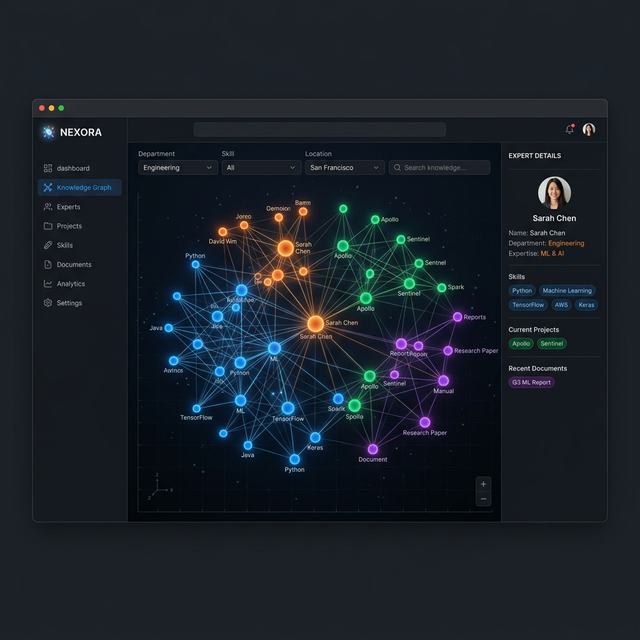
\includegraphics[width=0.85\textwidth]{maquettes/maquette_graphe.png}
    \caption{Visualisation 3D du graphe de connaissances}
\end{figure}

\textbf{Description :} Fonctionnalité centrale. Graphe 3D interactif (Three.js / WebGL) des experts, compétences, projets et documents.

\textbf{Composants :}
\begin{itemize}
    \item \textbf{Graphe 3D} — nœuds colorés : orange (Experts), bleu (Skills), vert (Projets), violet (Documents).
    \item \textbf{Barre de filtres} — Département, Compétence, Localisation.
    \item \textbf{Panneau de détails} — infos du nœud sélectionné.
\end{itemize}

\textbf{Interactions :} Clic = détails. Rotation/Zoom = navigation 3D. Filtres via \texttt{GET /api/graph/nodes}.

% ══════════════════════════════════════════════════════════════
\section{Learning Paths (Parcours d'Apprentissage)}
% ══════════════════════════════════════════════════════════════

\begin{verbatim}
  ┌──────────┬───────────────────────────────────┐
  │ SIDEBAR  │ My Learning Paths                 │
  │          │                                   │
  │          │ Vos lacunes identifiées :           │
  │          │ ┌─────────────────────────────┐   │
  │          │ │ Kubernetes  [████░░░░] 45%  │   │
  │          │ │ GraphQL     [███░░░░░] 35%  │   │
  │          │ │ Terraform   [██░░░░░░] 20%  │   │
  │          │ └─────────────────────────────┘   │
  │          │                                   │
  │          │ Parcours recommandé :               │
  │          │ ┌─────────────────────────────┐   │
  │          │ │ 1. Kubernetes Basics    [>] │   │
  │          │ │ 2. Container Orchestr.  [>] │   │
  │          │ │ 3. Helm Charts          [>] │   │
  │          │ └─────────────────────────────┘   │
  │          │                                   │
  │          │ Mentors suggérés :                  │
  │          │ [Av] Ahmed B. - Expert Kubernetes  │
  │          │ [Av] Li Wei  - Expert DevOps       │
  └──────────┴───────────────────────────────────┘
\end{verbatim}

\textbf{Description :} Page personnalisée basée sur le filtrage collaboratif. Identifie les lacunes et propose un parcours avec mentors.

\textbf{Composants :}
\begin{itemize}
    \item \textbf{Section Lacunes} — barres de progression des compétences manquantes.
    \item \textbf{Parcours recommandé} — liste ordonnée de sujets à apprendre.
    \item \textbf{Mentors suggérés} — experts internes qui maîtrisent ces compétences.
\end{itemize}

\textbf{Données :} \texttt{GET /api/ai/skill-gap} (filtrage collaboratif).

% ══════════════════════════════════════════════════════════════
\section{AI Insights (Intelligence Artificielle)}
% ══════════════════════════════════════════════════════════════

\begin{figure}[H]
    \centering
    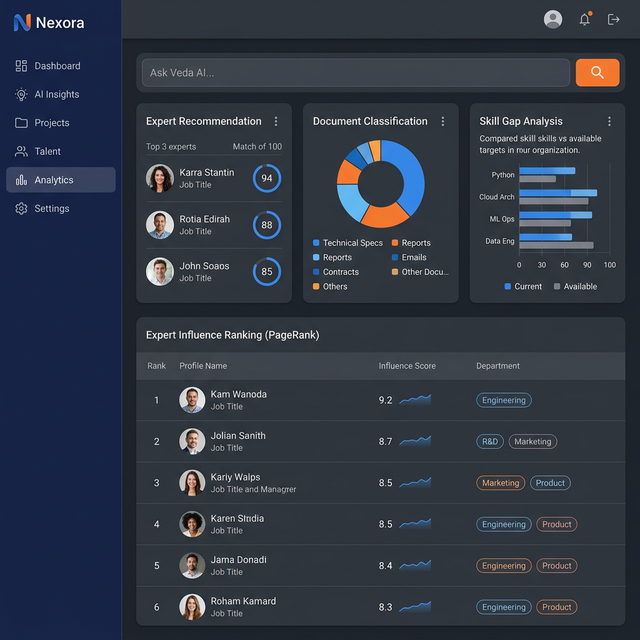
\includegraphics[width=0.85\textwidth]{maquettes/maquette_ai_insights.png}
    \caption{Page AI Insights — recommandations et analyses IA}
\end{figure}

\textbf{Description :} Toutes les fonctionnalités d'IA : recommandation, chatbot, classification, PageRank.

\textbf{Composants :}
\begin{itemize}
    \item \textbf{Barre de recherche Veda} — questions en langage naturel.
    \item \textbf{Recommandation d'Experts} — top experts avec score TF-IDF.
    \item \textbf{Classification de Documents} — répartition par catégorie.
    \item \textbf{Skill Gap Analysis} — barres horizontales des lacunes.
    \item \textbf{PageRank} — classement des experts par influence.
\end{itemize}

% ══════════════════════════════════════════════════════════════
\section{Skill Evolution (Tendances)}
% ══════════════════════════════════════════════════════════════

\begin{figure}[H]
    \centering
    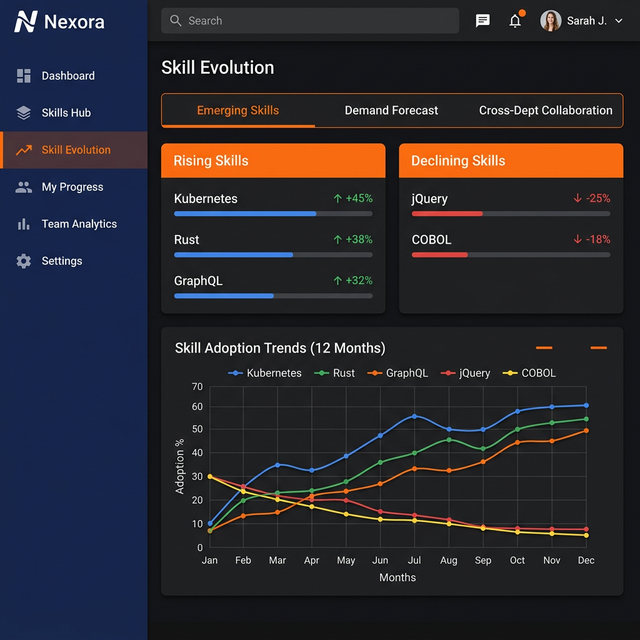
\includegraphics[width=0.85\textwidth]{maquettes/maquette_skill_evolution.png}
    \caption{Page Skill Evolution — tendances et prévisions}
\end{figure}

\textbf{Description :} Analyse des tendances de compétences pour les managers.

\textbf{Composants (3 onglets) :}
\begin{itemize}
    \item \textbf{Onglet 1 — Émergentes :} Skills en hausse (vert) et en déclin (rouge), analyse de cohortes.
    \item \textbf{Onglet 2 — Prévisions :} Projections à 6/12/18/24 mois avec niveaux d'urgence.
    \item \textbf{Onglet 3 — Collaboration :} Paires de départements complémentaires avec score.
\end{itemize}

% ══════════════════════════════════════════════════════════════
\section{Workspaces (Espaces de Travail)}
% ══════════════════════════════════════════════════════════════

\begin{verbatim}
  ┌──────────┬───────────┬───────────────────────┐
  │ SIDEBAR  │Workspaces │ Workspace: Project    │
  │          │           │ Nexus                 │
  │          │# Project  │                       │
  │          │  Nexus    │ Members: 5 [+ Invite] │
  │          │# Data     │                       │
  │          │  Pipeline │ Sarah: Les tests sont │
  │          │# Frontend │ passés!       15:01   │
  │          │  Team     │                       │
  │          │           │ Omar: Super, je merge │
  │          │[+ Create] │ la PR.        15:03   │
  │          │           │                       │
  │          │           │┌─────────────────────┐│
  │          │           ││ Message... [Envoyer] ││
  │          │           │└─────────────────────┘│
  └──────────┴───────────┴───────────────────────┘
\end{verbatim}

\textbf{Description :} Espaces de collaboration d'équipe avec chat temps réel via WebSocket.

\textbf{Composants :}
\begin{itemize}
    \item \textbf{Liste des workspaces} — canaux par projet/équipe.
    \item \textbf{Bouton Create} — création d'un nouveau workspace.
    \item \textbf{En-tête} — nom, nombre de membres, bouton inviter.
    \item \textbf{Zone de chat} — messages avec horodatage.
\end{itemize}

% ══════════════════════════════════════════════════════════════
\section{Dashboard (Tableau de Bord)}
% ══════════════════════════════════════════════════════════════

\begin{figure}[H]
    \centering
    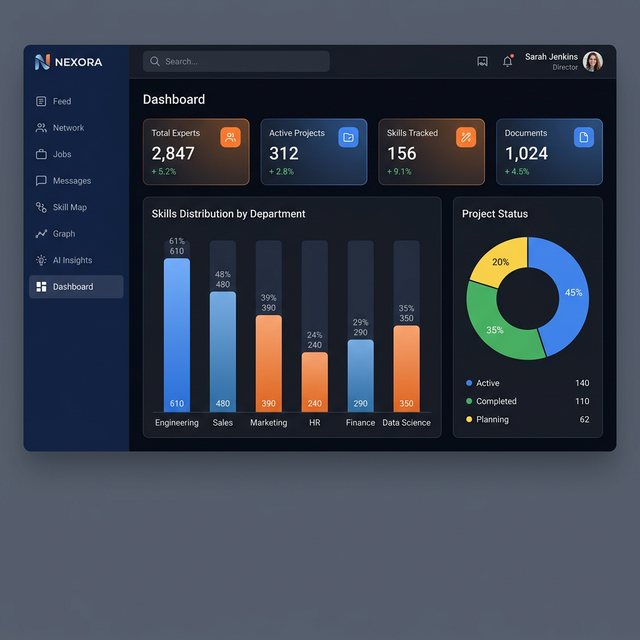
\includegraphics[width=0.85\textwidth]{maquettes/maquette_dashboard.png}
    \caption{Tableau de bord analytique}
\end{figure}

\textbf{Description :} Vue d'ensemble de l'organisation (accès Manager+).

\textbf{Composants :}
\begin{itemize}
    \item \textbf{4 cartes statistiques} — Total Experts, Projets Actifs, Skills, Documents.
    \item \textbf{Graphique en barres} — top compétences par département.
    \item \textbf{Graphique circulaire} — statut des projets (Actif, Terminé, Planifié).
\end{itemize}

\textbf{Données :} \texttt{GET /api/dashboard/stats}.

% ══════════════════════════════════════════════════════════════
\section{Résumé des Écrans}
% ══════════════════════════════════════════════════════════════

\begin{tabular}{|p{0.8cm}|p{4cm}|p{2.5cm}|p{6cm}|}
\hline
\textbf{N°} & \textbf{Page} & \textbf{Accès} & \textbf{Rôle principal} \\
\hline
1 & Login & Public & Authentification JWT \\
\hline
2 & Register & Public & Inscription nouveau compte \\
\hline
3 & Feed & User+ & Fil d'actualités, publications \\
\hline
4 & My Network & User+ & Réseau professionnel \\
\hline
5 & Jobs & User+ & Offres d'emploi internes \\
\hline
6 & Messaging & User+ & Chat privé entre utilisateurs \\
\hline
7 & Skill Map & User+ & Carte des compétences \\
\hline
8 & Team Builder & User+ & Composition d'équipes optimales \\
\hline
9 & Graph Explorer & User+ & Graphe 3D interactif \\
\hline
10 & Learning Paths & User+ & Parcours d'apprentissage personnalisé \\
\hline
11 & AI Insights & User+ & Recommandations IA, chatbot, PageRank \\
\hline
12 & Skill Evolution & Manager+ & Tendances et prévisions compétences \\
\hline
13 & Workspaces & User+ & Espaces de travail d'équipe \\
\hline
14 & Dashboard & Manager+ & Statistiques globales \\
\hline
\end{tabular}

\end{document}
